% Vorbereitung: Vorbereitungsaufgaben bearbeiten
% Versuchsaufbau: Verwendete Apparatur, Beschreibung Funktionsweise/Nutzen mit Skizze/Foto
\section{Durchführung}
\label{sec:durchführung}
Im Folgenden wird die Versuchsdurchführung und der Aufbau beschrieben und erläutert.

\subsection{Versuchsaufbau}
\label{sec:Versuchsaufbau}

\autoref{fig:aufbau} zeigt eine schematische Darstellung des verwendeten Versuchsaufbaus.
\begin{figure}[H]
    \centering
    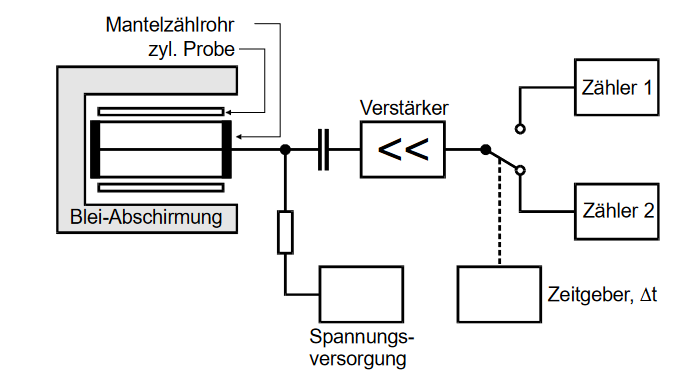
\includegraphics[width=0.8\linewidth]{content/grafik/aufbau.png}
    \caption{Schematischer Versuchsaufbau.\cite{neutron}}
    \label{fig:aufbau}
\end{figure}

Die aktivierte Probe wird auf das Geiger-Müller Zählrohr gesteckt. Mittels einer Blei-Abschirmung wird die 
Umgebungsradioaktivität möglichst gering gehalten. Die gemessenen Teilchen liefern am Verstärkungsausgang einen elektrischen 
Impuls. Das benutzte Zählwerk erhält diese Impulse. Das Zählwerk schaltet periodisch pro gewähltem Zeitintervall
von Zähler 1 zu Zähler 2  und umgekehrt.

\subsection{Versuchsdurchführung}
\label{sec:Versuchsdurchführung}

Als erstes wurde eine Nullmessung durchgeführt, um den Nulleffekt zu bestimmen. In einem Zeitintervall von $t = \SI{600}{\second}$
wurde alle $\SI{10}{\second}$ die Zählrate der Umgebung gemessen.
Bei den Proben ist es zu beachten, dass diese relativ zügig aus dem Paraffinbehälter entfernt werden müssen, um dann auf 
das Zählrohr gesteckt zu werden. Zunächst wird die erste Messreihe für Rhodium aufgenommen, indem für 12 Minuten alle $\SI{8}{\second}$
die Zählrate gemessen wird. In dem Zeitraum, in dem die Rhodium Probe erneut aktiviert wird, wird in einem Zeitraum von 15 Minuten
alle $\SI{30}{\second}$ die Zählrate von Vanadium aufgenommen. Anschließend wird die zweite Messung für die Rhodium Probe durchgeführt.
